\documentclass[11pt]{scrartcl}
\usepackage[utf8]{inputenc}
\usepackage{mathtools}
\usepackage{amssymb}
\usepackage{listings}
\usepackage{bm}
\usepackage{graphicx}
\usepackage{xcolor}
\usepackage{qtree}
\usepackage{tikz}
\lstset
{ %Formatting for code in appendix
	language=Matlab,
	basicstyle=\footnotesize,
	numbers=left,
	stepnumber=1,
	showstringspaces=true,
	tabsize=1,
	breaklines=true,
	breakatwhitespace=false,
}
\begin{document}
\centerline{\LARGE{\textbf{CSE881 HW7}}}
\centerline{\large{\textit{Nan Cao,\  A52871775}}}
\centerline{\large{\textit{Nov 6th, 2016}}}

\section*{Problem 1}
\textbf{(a)}\\

$$<\{r\},\{p,q\}>$$
$$<\{p,q\},\{r\}>$$
$$<\{p,q\},\{p\}>$$
$$<\{p,q\},\{q\}>$$
$$<\{p\},\{p,q\}>$$
$$<\{q\},\{p,q\}>$$
$$<\{p\},\{r\},\{p\}>$$
$$<\{p\},\{r\},\{q\}>$$
$$<\{q\},\{r\},\{p\}>$$
$$<\{q\},\{r\},\{q\}>$$
\textbf{(b)}\\
$$<\{p\},\{r\},\{p\}>$$
$$<\{p\},\{r\},\{q\}>$$
$$<\{q\},\{r\},\{p\}>$$
$$<\{q\},\{r\},\{q\}>$$
$$<\{p,q\},\{r\},\{p\}>$$
$$<\{p,q\},\{r\},\{q\}>$$
$$<\{p\},\{r\},\{p,q\}>$$
$$<\{q\},\{r\},\{p,q\}>$$
$$<\{p,q\},\{r\},\{p,q\}>$$
\newpage
\textbf{(c)}\\
$$<\{p,q,r\},\{s\}>$$%2,5
$$<\{p,r,s\},\{s\}>$$%1
$$<\{p\},\{p,q,r\}>$$%3,2
$$<\{p\},\{p,q\},\{s\}>$$%2,2
$$<\{p,q\},\{s\},\{p\}>$$%2,2
$$<\{q\},\{r,s\},\{s\}>$$%2
$$<\{q,r\},\{s\},\{s\}>$$%1

\textbf{(d)}
$$<\{p,q,r\},\{s\}>$$%2,5
\section*{Problem 2}
\textbf{(a)}\\
$w=<\{p\}\{q\}\{r\}\{s\}\{t\} >$\\
Yes\\
$w=< \{p\}\{p\}\{q\}\{q\} >$\\
Yes\\
$w=< \{p\}\{s\}\{t\} >$\\
No\\
$w=< \{p, r\}\{q, r\}\{q, s\} >$\\
No\\
\textbf{(b)}\\
$w =< \{p, q, r, s, t\} >$\\
Yes\\
$w =< \{q,r, s, t\}\{q,r\}\{q,s\} >$\\
Yes\\
$w =< \{r, s\}\{r, s\}\{r, s\} >$\\
No\\
$w =< \{p, q, r\}\{q, r, s\} >$\\
No\\
\section*{Problem 3}
\textbf{(a)}\\
% \begin{tikzpicture}[
% roundnode/.style={circle, draw=green!60, fill=green!5, very thick, minimum size=7mm},
% squarednode/.style={rectangle, draw=red!60, fill=red!5, very thick, minimum size=5mm},
% ]
% %Nodes
\begin{tikzpicture}
\node (1) at ( 0,1)[circle,draw,fill=green!30] {a};
\node (2) at ( 0,0) [circle,draw,fill=green!30] {b};
\node (3) at ( 0,-1) [circle,draw,fill=green!30] {a};
\node (4) at ( 1,1)[circle,draw] {a};
\node (5) at ( 1,0) [circle,draw,fill=green!30] {b};
\node (6)at ( 1,-1) [circle,draw] {a};
\draw  (1) -- (2);
\draw  (2) -- (3);
\draw  (2) -- (5);
\draw  (4) -- (5);
\draw  (5) -- (6);
\end{tikzpicture}
\ \ \ \ \ 
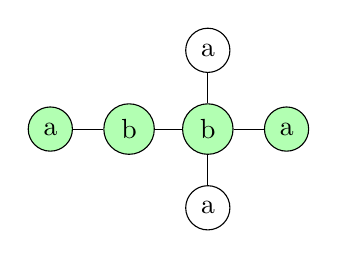
\begin{tikzpicture}
\node (1) at ( 0,0) [circle,draw,fill=green!30] {a};
\node (2) at ( 1,0) [circle,draw,fill=green!30] {b};
\node (3) at ( 2,0) [circle,draw,fill=green!30] {b};
\node (4) at ( 3,0) [circle,draw,fill=green!30] {a};
\node (5) at ( 2,1) [circle,draw] {a};
\node (6)at ( 2,-1) [circle,draw] {a};
\draw  (1) -- (2);
\draw  (2) -- (3);
\draw  (3) -- (4);
\draw  (3) -- (5);
\draw  (3) -- (6);
\end{tikzpicture}
\ \ \ \ \ 
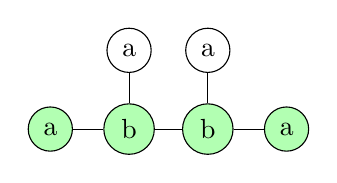
\begin{tikzpicture}
\node (1) at ( 0,0) [circle,draw,fill=green!30] {a};
\node (2) at ( 1,0) [circle,draw,fill=green!30] {b};
\node (3) at ( 2,0) [circle,draw,fill=green!30] {b};
\node (4) at ( 3,0) [circle,draw,fill=green!30] {a};
\node (5) at ( 2,1) [circle,draw] {a};
\node (6)at ( 1,1) [circle,draw] {a};
\draw  (1) -- (2);
\draw  (2) -- (3);
\draw  (3) -- (4);
\draw  (3) -- (5);
\draw  (2) -- (6);
\end{tikzpicture}
\ \ \ \ \ 
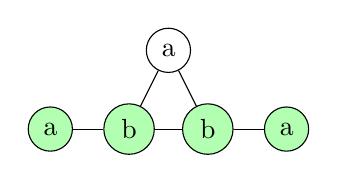
\begin{tikzpicture}
\node (1) at ( 0,0) [circle,draw,fill=green!30] {a};
\node (2) at ( 1,0) [circle,draw,fill=green!30] {b};
\node (3) at ( 2,0) [circle,draw,fill=green!30] {b};
\node (4) at ( 3,0) [circle,draw,fill=green!30] {a};
\node (5) at ( 1.5,1) [circle,draw] {a};
\draw  (1) -- (2);
\draw  (2) -- (3);
\draw  (3) -- (4);
\draw  (2) -- (5);
\draw  (3) -- (5);
\end{tikzpicture}
\\
\textbf{(b)}\\
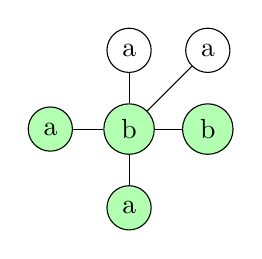
\begin{tikzpicture}
\node (1) at ( 0,0) [circle,draw,fill=green!30] {a};
\node (2) at ( 1,0) [circle,draw,fill=green!30] {b};
\node (3) at ( 2,0) [circle,draw,fill=green!30] {b};
\node (4) at ( 1,-1) [circle,draw,fill=green!30] {a};
\node (5) at ( 1,1) [circle,draw] {a};
\node (6)at ( 2,1) [circle,draw] {a};
\draw  (1) -- (2);
\draw  (2) -- (3);
\draw  (2) -- (4);
\draw  (2) -- (5);
\draw  (2) -- (6);
\end{tikzpicture}
\ \ \ \ \ 
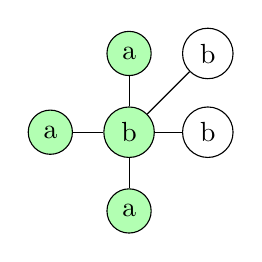
\begin{tikzpicture}
\node (1) at ( 0,0) [circle,draw,fill=green!30] {a};
\node (2) at ( 1,0) [circle,draw,fill=green!30] {b};
\node (3) at ( 2,0) [circle,draw] {b};
\node (4) at ( 1,-1) [circle,draw,fill=green!30] {a};
\node (5) at ( 1,1) [circle,draw,fill=green!30] {a};
\node (6)at ( 2,1) [circle,draw] {b};
\draw  (1) -- (2);
\draw  (2) -- (3);
\draw  (2) -- (4);
\draw  (2) -- (5);
\draw  (2) -- (6);
\end{tikzpicture}
\\
\textbf{(c)}\\
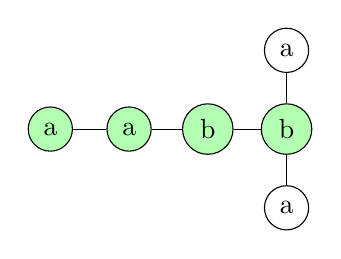
\begin{tikzpicture}
\node (1) at ( 0,0) [circle,draw,fill=green!30] {a};
\node (2) at ( 1,0) [circle,draw,fill=green!30] {a};
\node (3) at ( 2,0) [circle,draw,fill=green!30] {b};
\node (4) at ( 3,0) [circle,draw,fill=green!30] {b};
\node (5) at ( 3,1) [circle,draw] {a};
\node (6)at ( 3,-1) [circle,draw] {a};
\draw  (1) -- (2);
\draw  (2) -- (3);
\draw  (3) -- (4);
\draw  (4) -- (5);
\draw  (4) -- (6);
\end{tikzpicture}
\ \ \ \ \ 
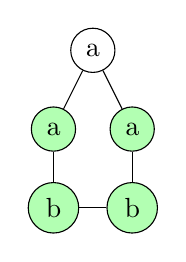
\begin{tikzpicture}
\node (1) at ( 0,0) [circle,draw,fill=green!30] {b};
\node (2) at ( 1,0) [circle,draw,fill=green!30] {b};
\node (3) at ( 0,1) [circle,draw,fill=green!30] {a};
\node (4) at ( 1,1) [circle,draw,fill=green!30] {a};
\node (5) at ( 0.5,2) [circle,draw] {a};
\draw  (1) -- (2);
\draw  (1) -- (3);
\draw  (2) -- (4);
\draw  (3) -- (5);
\draw  (4) -- (5);
\end{tikzpicture}
\ \ \ \ \ 
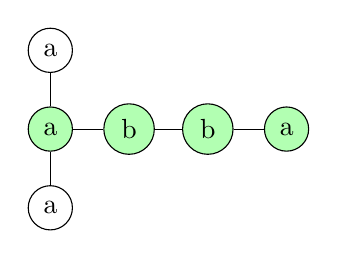
\begin{tikzpicture}
\node (1) at ( 0,0) [circle,draw,fill=green!30] {a};
\node (2) at ( 1,0) [circle,draw,fill=green!30] {b};
\node (3) at ( 2,0) [circle,draw,fill=green!30] {b};
\node (4) at ( 3,0) [circle,draw,fill=green!30] {a};
\node (5) at ( 0,1) [circle,draw] {a};
\node (6) at ( 0,-1) [circle,draw] {a};
\draw  (1) -- (2);
\draw  (2) -- (3);
\draw  (3) -- (4);
\draw  (1) -- (5);
\draw  (1) -- (6);
\end{tikzpicture}
\ \ \ \ \ 
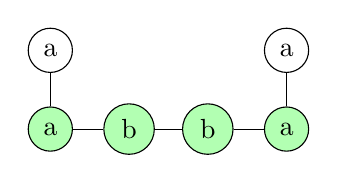
\begin{tikzpicture}
\node (1) at ( 0,0) [circle,draw,fill=green!30] {a};
\node (2) at ( 1,0) [circle,draw,fill=green!30] {b};
\node (3) at ( 2,0) [circle,draw,fill=green!30] {b};
\node (4) at ( 3,0) [circle,draw,fill=green!30] {a};
\node (5) at ( 0,1) [circle,draw] {a};
\node (6) at ( 3,1) [circle,draw] {a};
\draw  (1) -- (2);
\draw  (2) -- (3);
\draw  (3) -- (4);
\draw  (1) -- (5);
\draw  (4) -- (6);
\end{tikzpicture}
\\
\textbf{(d)}\\
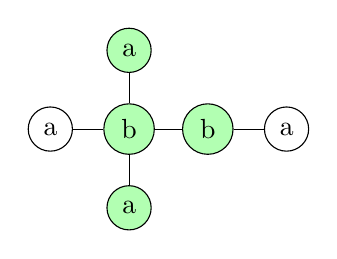
\begin{tikzpicture}
\node (1) at ( 0,0) [circle,draw] {a};
\node (2) at ( 1,0) [circle,draw,fill=green!30] {b};
\node (3) at ( 2,0) [circle,draw,fill=green!30] {b};
\node (4) at ( 3,0) [circle,draw] {a};
\node (5) at ( 1,1) [circle,draw,fill=green!30] {a};
\node (6) at ( 1,-1) [circle,draw,fill=green!30] {a};
\draw  (1) -- (2);
\draw  (2) -- (3);
\draw  (3) -- (4);
\draw  (2) -- (5);
\draw  (2) -- (6);
\end{tikzpicture}
\ \ \ \ \ 
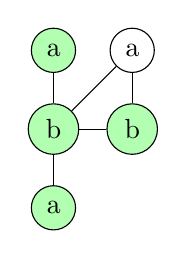
\begin{tikzpicture}
\node (1) at ( 0,0)[circle,draw,fill=green!30] {b};
\node (2) at ( 1,0) [circle,draw,fill=green!30] {b};
\node (3) at ( 0,1) [circle,draw,fill=green!30] {a};
\node (4) at ( 0,-1) [circle,draw,fill=green!30] {a};
\node (5) at ( 1,1)[circle,draw] {a};
\draw  (1) -- (2);
\draw  (1) -- (3);
\draw  (1) -- (4);
\draw  (2) -- (5);
\draw  (1) -- (5);
\end{tikzpicture}
\\
\textbf{(e)}\\
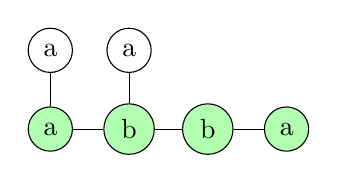
\begin{tikzpicture}
\node (1) at ( 0,0) [circle,draw,fill=green!30] {a};
\node (2) at ( 1,0) [circle,draw,fill=green!30] {b};
\node (3) at ( 2,0) [circle,draw,fill=green!30] {b};
\node (4) at ( 3,0) [circle,draw,fill=green!30] {a};
\node (5) at ( 0,1) [circle,draw] {a};
\node (6) at ( 1,1) [circle,draw] {a};
\draw  (1) -- (2);
\draw  (2) -- (3);
\draw  (3) -- (4);
\draw  (1) -- (5);
\draw  (2) -- (6);
\end{tikzpicture}
\ \ \ \ \ 
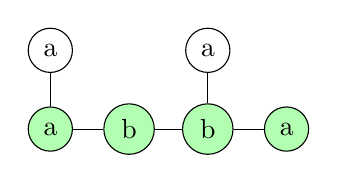
\begin{tikzpicture}
\node (1) at ( 0,0) [circle,draw,fill=green!30] {a};
\node (2) at ( 1,0) [circle,draw,fill=green!30] {b};
\node (3) at ( 2,0) [circle,draw,fill=green!30] {b};
\node (4) at ( 3,0) [circle,draw,fill=green!30] {a};
\node (5) at ( 0,1) [circle,draw] {a};
\node (6) at ( 2,1) [circle,draw] {a};
\draw  (1) -- (2);
\draw  (2) -- (3);
\draw  (3) -- (4);
\draw  (1) -- (5);
\draw  (3) -- (6);
\end{tikzpicture}
\ \ \ \ \ 
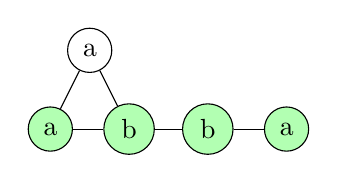
\begin{tikzpicture}
\node (1) at ( 0,0) [circle,draw,fill=green!30] {a};
\node (2) at ( 1,0) [circle,draw,fill=green!30] {b};
\node (3) at ( 2,0) [circle,draw,fill=green!30] {b};
\node (4) at ( 3,0) [circle,draw,fill=green!30] {a};
\node (5) at ( 0.5,1) [circle,draw] {a};
\draw  (1) -- (2);
\draw  (2) -- (3);
\draw  (3) -- (4);
\draw  (1) -- (5);
\draw  (2) -- (5);
\end{tikzpicture}
\ \ \ \ \ 
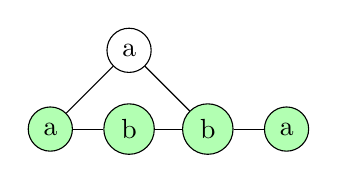
\begin{tikzpicture}
\node (1) at ( 0,0) [circle,draw,fill=green!30] {a};
\node (2) at ( 1,0) [circle,draw,fill=green!30] {b};
\node (3) at ( 2,0) [circle,draw,fill=green!30] {b};
\node (4) at ( 3,0) [circle,draw,fill=green!30] {a};
\node (5) at ( 1,1) [circle,draw] {a};
\draw  (1) -- (2);
\draw  (2) -- (3);
\draw  (3) -- (4);
\draw  (1) -- (5);
\draw  (3) -- (5);
\end{tikzpicture}
\\
\textbf{(f)}\\
No candidates.
%Lines
% \draw[->] (uppercircle.south) -- (maintopic.north);
% \draw[->] (maintopic.east) -- (rightsquare.west);
% \draw[->] (rightsquare.south) .. controls +(down:7mm) and +(right:7mm) .. (lowercircle.east);
% \end{tikzpicture}
\end{document}